\documentclass[mathNotesPreamble]{subfiles}
\begin{document}
%\relscale{1.4} %TODO
\section{17.6: Surface Integrals}

  Imagine a sphere with a known temperature distribution. How would we find the average temperature over the sphere?
  \vspace*{\stretch{1}}

  \begin{center}
    \begin{tabular}{@{}l@{\hspace*{25pt}}l@{}}\toprule
      \multicolumn{2}{c}{\textbf{Parallel Concepts}}\\\midrule
      \textbf{Curves}& \textbf{Surfaces}\\
      Arc length& Surface area\\
      Line integrals& Surface integrals\\
      One-parameter description& Two-parameter description\\\bottomrule
    \end{tabular}
  \end{center}
  \vspace*{\stretch{1}}

  \noindent
  \textbf{Parameterized Surfaces}

  Recall that in $\bbr^2$, we parameterized a curve by $\vecr(t)=\bracket{x(t),\,y(t)}$ where $a\leq t\leq b$. In $\bbr^3$, we parameterize a surface by 
    \[\vecr(u,v)=\bracket{x(u,v),\,y(u,v),\,z(u,v)}\]
  where the parameters are over $R=\set{(u,v): a\leq u\leq b, c\leq v\leq d}$
  \vspace*{\stretch{1}}
  \begin{center}
    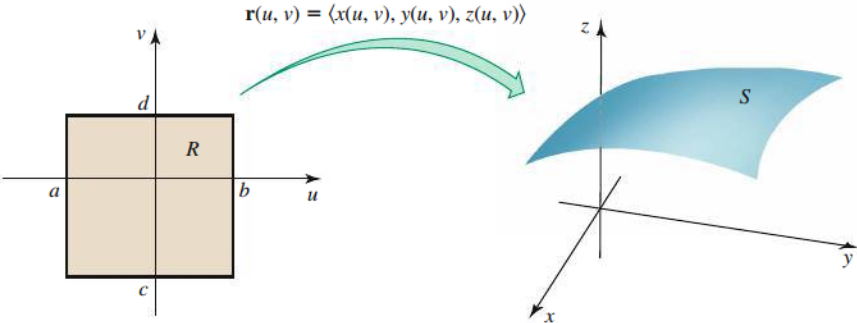
\includegraphics[width=0.85\linewidth]{images/briggs_17_06/fig17_43}
  \end{center}
  \pagebreak

  \textbf{Cylinders:}
    \[\set{(x,\,y,\,z): x=a\cos(\theta),\,y=a\sin(\theta),\ 0\leq\theta\leq 2\pi,\, 0\leq z\leq h}\]
    \[\vecr(u,v)=\bracket{x(u,v),\,y(u,v),\,z(u,v)}=\bracket{a\cos(u),\,a\sin(u),\,v}\]
  \begin{center}
    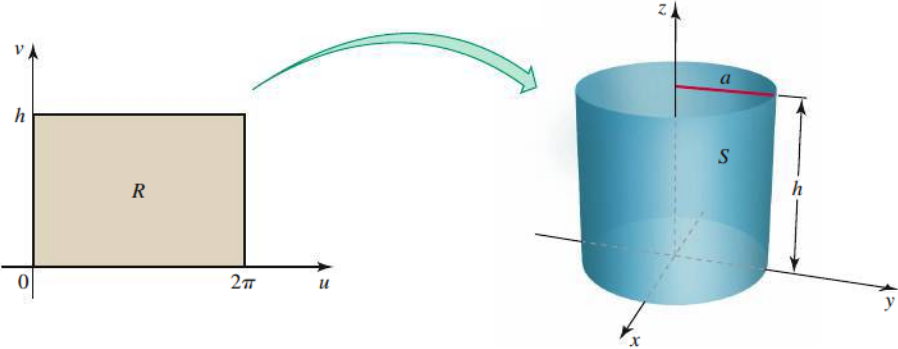
\includegraphics[width=0.7\linewidth]{images/briggs_17_06/fig17_44}
  \end{center}
  \vspace*{\stretch{1}}

  \textbf{Cones:}
  \[\set{(r,\,\theta,\,z): 0\leq r\leq a,\, 0\leq\theta\leq 2\pi,\, z=rh/a}\]
  For a fixed value of $z$, $r=az/h$:
    \[x=r\cos(\theta)=\frac{az}{h}\cos(\theta) \textnormal{ and } y=r\sin(\theta)=\frac{az}{h}\sin(\theta)\]
  Now, let $u=\theta$ and $v=z$, then
    \[\vecr(u,v)=\bracket{x(u,v),\,y(u,v),\,z(u,v)}=\bracket{\frac{av}{h}\cos(u),\,\frac{av}{h}\sin(u),\,v}\]
  \begin{center}
    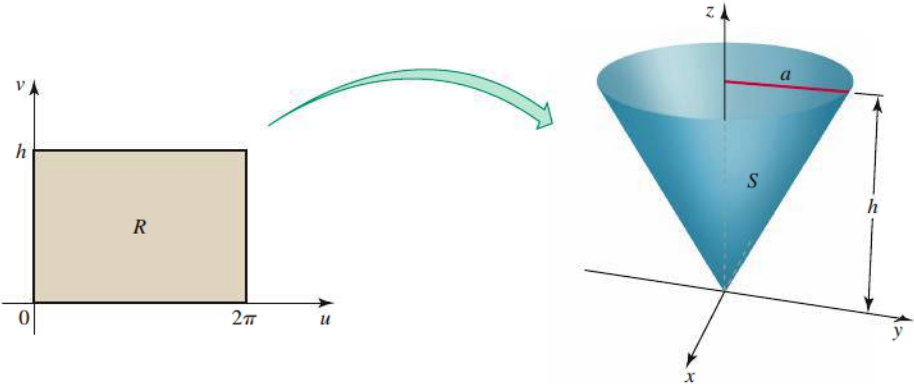
\includegraphics[width=0.7\linewidth]{images/briggs_17_06/fig17_45}
  \end{center}
  \vspace*{\stretch{1}}
  \pagebreak

  \textbf{Spheres:}
  \[\set{(\rho,\,\varphi,\,\theta): \rho=a, 0\leq \varphi\leq \pi,\, 0\leq\theta\leq 2\pi}\]

  \[x=a\sin(\varphi)\cos(\theta), \qquad y=a\sin(\varphi)\sin(\theta), \qquad z=a\cos(\varphi)\]
  Now, let $u=\theta$ and $v=z$, then
    \[\vecr(u,v)=\bracket{x(u,v),\,y(u,v),\,z(u,v)}=\bracket{a\sin(u)\cos(v),\,a\sin(u)\cos(v),\,a\cos(u)}\]
  \begin{center}
    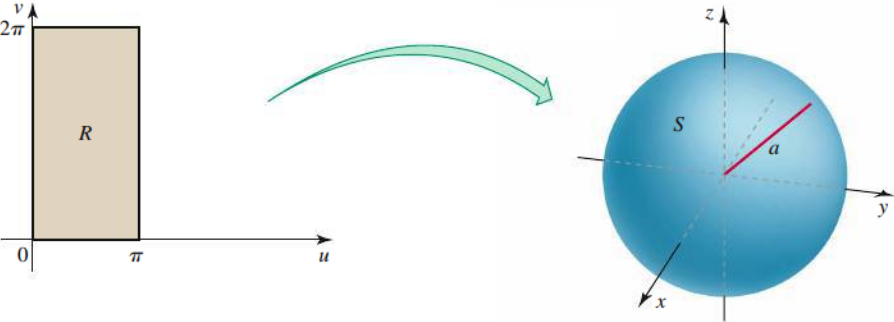
\includegraphics[width=0.7\linewidth]{images/briggs_17_06/fig17_46}
  \end{center}
  \vspace*{0.5\baselineskip}

  \begin{ex*}
    Find parametric descriptions for the following surfaces
  \end{ex*}
  \begin{tasks}[after-item-skip=\stretch{1}, label=](1)
    \task The plane $3x-2y+z=2$
    \task The paraboloid $z=x^2+y^2$, for $0\leq z\leq 9$
  \end{tasks}
  \vspace*{\stretch{1}}
  \pagebreak

  \noindent
  \textbf{Surface Integrals  of Scalar-Valued Functions}

  \begin{center}
    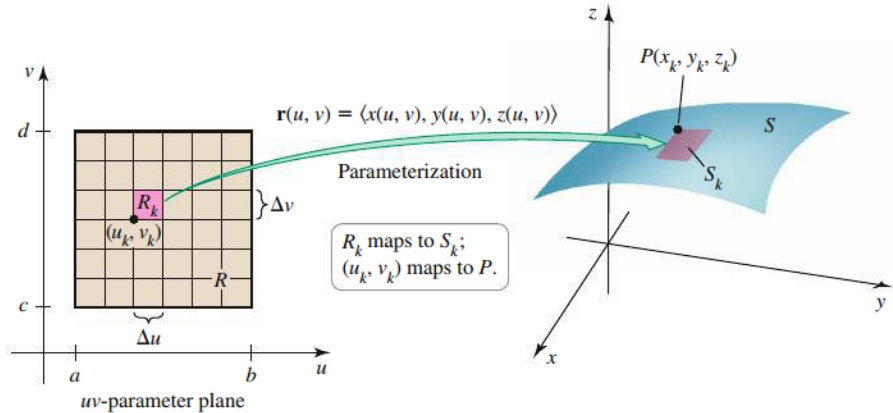
\includegraphics[width=0.8\linewidth]{images/briggs_17_06/fig17_47}
  \end{center}
  \vspace*{\stretch{1}}
  Using the parameterization 
    \[\vecr(u,v)=\bracket{x(u,v),\, y(u,v),\,z(u,v)}\]
  over the region $R=\set{(u,v): a\leq u\leq b,\, c\leq v\leq d}$, it is important that we know $\Delta S_k$, which is the area of $S_k$.
  \vspace*{\stretch{1}}
  \begin{center}
    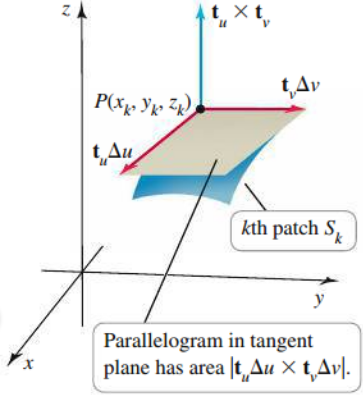
\includegraphics[width=0.35\linewidth]{images/briggs_17_06/fig17_48}
  \end{center}
  \pagebreak

  \begin{defn*}[Surface Integral of Scalar-Valued Functions on Parameterized Surfaces]
    Let $f$ be a continuous scalar-valued function on a smooth surface $S$ given parametrically by $\vecr(u,v)=\bracket{x(u,v),\,y(u,v),\,z(u,v)}$, where $u$ and $v$ vary over \newline$R=\set{(u,v): a\leq u\leq b,\, c\leq v\leq d}$. Assume also that the tangent vectors \newline
      \[\displaystyle \mathbf t_u=\frac{\partial \vecr}{\partial u}=\bracket{\frac{\partial x}{\partial u},\, \frac{\partial y}{\partial u},\, \frac{\partial z}{\partial u}}
      \textnormal{ and }
      \displaystyle\mathbf t_v=\frac{\partial \vecr}{\partial v}=\bracket{\frac{\partial x}{\partial v},\, \frac{\partial y}{\partial v},\, \frac{\partial z}{\partial v}}\]
    are continuous on $R$ and the normal vector $\mathbf t_u\times\mathbf t_v$ is nonzero on $R$. Then the \textbf{surface integral of $f$ over $S$} is 
      \[\iint\limits_S f(x,y,z)\,dS = \iint\limits_R f\parens{x(u,v),\,y(u,v),\,z(u,v)}\abs{\mathbf t_u\times\mathbf t_v}\,dA\]
    If $f(x,y,z)=1$, this integral equals the surface area of $S$.
  \end{defn*}
  \begin{ex*}
    Find the surface area of the following surfaces
  \end{ex*}
  \begin{tasks}[after-item-skip=\stretch{1}, label=](1)
    \task A cylinder with radius $a>0$ and height $h$ (open ends)
  \end{tasks}
  \vspace*{\stretch{1}}
  \pagebreak

  \begin{tasks}[after-item-skip=\stretch{1}, label=, resume](1)
    \task A sphere of radius $a$
  \end{tasks}
  \vspace*{\stretch{1}}
  \pagebreak

  \begin{ex*}
    The temperature on the surface of a sphere of radius $a$ varies with latitude according to the function $T(\varphi, \theta)=10+50\sin(\varphi)$, for $0\leq \varphi\leq \pi$ and $0\leq \theta\leq 2\pi$. Find the average temperature over the sphere.
  \end{ex*}
  \vspace*{\stretch{1}}
  \pagebreak

  \noindent
  \textbf{Surface Integrals on Explicitly Defined Surfaces}

  Suppose a smooth surface $S$ is defined explicitly as $z=g(x,y)$. Here, we let $u=x$ and $v=y$. This gives us
    \[\mathbf t_u=\mathbf t_x=\bracket{1,\,0,\,z_x},\quad \mathbf t_v=\mathbf t_y=\bracket{0,\,1,\,z_y}\]
  thus
    \[\mathbf t_x\times\mathbf t_y=\bracket{-z_x,\,-z_y,\,1}\]
  and
    \[\abs{\mathbf t_x\times\mathbf t_y}=\sqrt{z^2_x+z^2_y+1}\]
  \vspace*{\stretch{0.5}}

  \begin{thmBox*}[Theorem 17.14: Evaluation of Surface Integrals of Scalar-Valued Functions on Explicitly Defined Surfaces]
    Let $f$ be a continuous function on a smooth surface $S$ given by $z=g(x,y)$, for $(x,y)$ in a region $R$. The surface integral of $f$ over $S$ is
      \[\iint\limits_S f(x,y,z)\,dS=\iint\limits_S f\parens{x,y,g(x,y)}\sqrt{z_x^2+z_y^2+1}\,dA.\]
    If $f(x,y,z)=1$, the surface integral equals the area of the surface.
  \end{thmBox*}
  \vspace*{\stretch{1}}
  \pagebreak

  \begin{ex*}
    Find the area of the surface $S$ that lies in the plane $z=12-4x-3y$ directly above the region $R$ bounded by the ellipse $x^2/4+y^2=1$
  \end{ex*}
  \begin{flushright}
    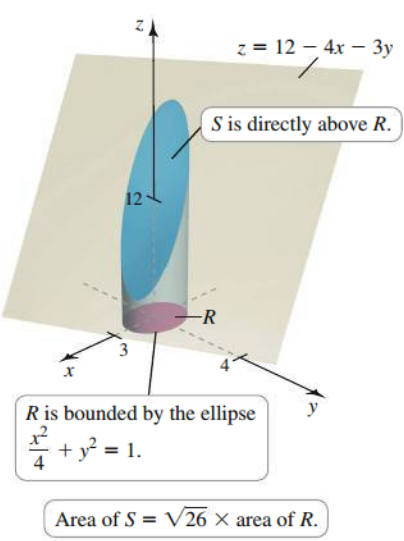
\includegraphics[width=0.3\linewidth]{images/briggs_17_06/fig17_53}
  \end{flushright}
  \vspace*{\stretch{1}}
  \pagebreak

  \begin{ex*}
    A thin conical sheet is described by the surface $z=\parens{x^2+y^2}^{\frac{1}{2}}$, for $0\leq z\leq 4$. The density of the sheet in $\textnormal{g/ cm}^2$ is $\rho=f(x,y,z)=(8-z)$. What is the mass of the cone?
  \end{ex*}
  \begin{flushright}
    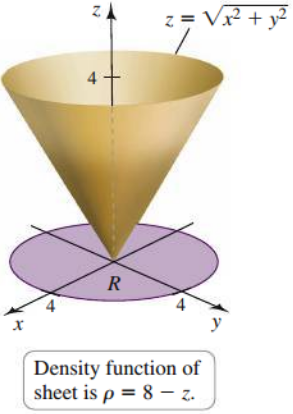
\includegraphics[width=0.25\linewidth]{images/briggs_17_06/fig17_54}
  \end{flushright}
  \vspace*{\stretch{1}}
  \pagebreak

  \begin{landscape}
  \vspace*{\stretch{1}}
%    \begin{center}
      \relscale{0.6}
      \renewcommand{\arraystretch}{1.85}
      \hspace*{-25pt}
      \begin{tabular}{@{}m{17.5mm}m{25mm}m{26.5mm}m{25mm}@{\hspace*{7.5mm}}m{42.5mm}m{40mm}m{18mm}@{}}\toprule
        \multicolumn{4}{c}{\textbf{Explicit Description $z=g(x,y)$}}& \multicolumn{3}{c}{\textbf{Parametric Description}}\\
          \textbf{Surface}& \textbf{Equation}& 
          \textbf{Normal vector}\newline $\pm\bracket{-z_x,\,-z_y,\,1}$&
          \textbf{magnitude}\newline $\abs{\bracket{-z_x,\,-z_y,\,1}}$&
          \textbf{Equation}&
          \textbf{Normal vector}\newline $\mathbf t_u\times \mathbf t_v$&
          \textbf{magnitude}\newline $\abs{\mathbf t_u\times\mathbf t_v}$\\\midrule
          %
          \textbf{Cylinder}& $x^2+y^2=a^2$,\newline $0\leq z\leq h$&
          $\bracket{x,y,0}$& $a$& 
          $\vecr=\bracket{a\cos(u),\,a\sin(u),\,v}$,\newline $0\leq u\leq 2\pi$, $0\leq v\leq h$& $\bracket{a\cos(u),\,a\sin(u),\,0}$& $a$\\
          %
          \textbf{Cone}& $z^2=x^2+y^2$,\newline $0\leq z\leq h$& $\bracket{x/z,\,y/z,\,-1}$& $\sqrt{2}$& 
          $\vecr=\bracket{v\cos(u),\,v\sin(u),\,v}$,\newline $0\leq u\leq 2\pi$, $0\leq v\leq h$& $\bracket{v\cos(u),\,v\sin(u),\,-v}$& $\sqrt{2}v$\\
          %
          \textbf{Sphere}& $x^2+y^2+z^2=a^2$& $\bracket{x/z,\,y/z,\,1}$;& $a/z$&
          $\vecr=\langle a\sin(u)\cos(v),$\newline \hspace*{8mm} $a\sin(u)\sin(v),$\newline \hspace*{19mm}$a\cos(u)\rangle$\newline $0\leq u\leq \pi$, $0\leq v\leq 2\pi$&
          $\langle a^2\sin^2(u)\cos(v)$, \hspace*{2mm}$a^2\sin^2(u)\sin(v)$, \hspace*{2.5mm}$a^2\sin(u)\cos(u)\rangle$& $a^2\sin(u)$\\
          %
          \textbf{Paraboloid}& $z=x^2+y^2$,\newline $0\leq z\leq h$& $\bracket{2x,\,2y,\,-1}$& $\sqrt{1+4(x^2+y^2)}$&
          $\vecr=\bracket{v\cos(u),\,v\sin(u),\,v^2}$,\newline $0\leq u\leq 2\pi$, $0\leq v\leq \sqrt{h}$& $\bracket{2v^2\cos(u),2v^2\sin(u),-v}$& $v\sqrt{1+4v^2}$\\\bottomrule
        \end{tabular}
%    \end{center}
  \vspace*{\stretch{1}}
  \end{landscape}

  \noindent
  \textbf{Surface Integrals of Vector Fields:}

  The surfaces we consider must be 
  \begin{itemize}
    \item \textbf{two-sided} or \textbf{orientable}
    \item \textbf{oriented}
  \end{itemize}
  

  \begin{defn*}[Surface Integral of a Vector Field]
    Suppose $\mathbf F=\bracket{f,\,g,\,h}$ is a continuous vector field on a region of $\bbr^3$ containing a smooth oriented surface $S$. If $S$ is defined parametrically as $\vecr(u,v)=\bracket{x(u,v),y(u,v),z(u,v)}$, for $(u,v)$ in a region $R$, then
      \[\iint\limits_S \mathbf F\cdot\vecn\,ds = \iint\limits_R \mathbf F\cdot\parens{\mathbf t_u\times\mathbf t_v}\,dA,\]
    where 
      \[\displaystyle\mathbf t_u=\frac{\partial \vecr}{\partial u}=\bracket{\frac{\partial x}{\partial u},\,\frac{\partial y}{\partial u},\,\frac{\partial z}{\partial u}}
      \textnormal{ and }
      \displaystyle\mathbf t_v=\frac{\partial \vecr}{\partial v}=\bracket{\frac{\partial x}{\partial v},\,\frac{\partial y}{\partial v},\,\frac{\partial z}{\partial v}}\] 
    and continuous on $R$, the normal vector $\mathbf t_u\times\mathbf t_v$ is nonzero on $R$, and the direction of the normal vector is consistent with the orientation of $S$. If $S$ is defined in the form $z=s(x,y)$, for $(x,y)$ in a region $R$, then 
      \[\iint\limits_S \mathbf F\cdot\vecn\,dS=\iint\limits_S \parens{-fz_x-gz_y+h}\,dA.\]
  \end{defn*}
  \pagebreak

  \textbf{Flux Integrals:}
    \[\iint\limits_S \mathbf F\cdot\vecn\,dS\]
  \begin{center}
    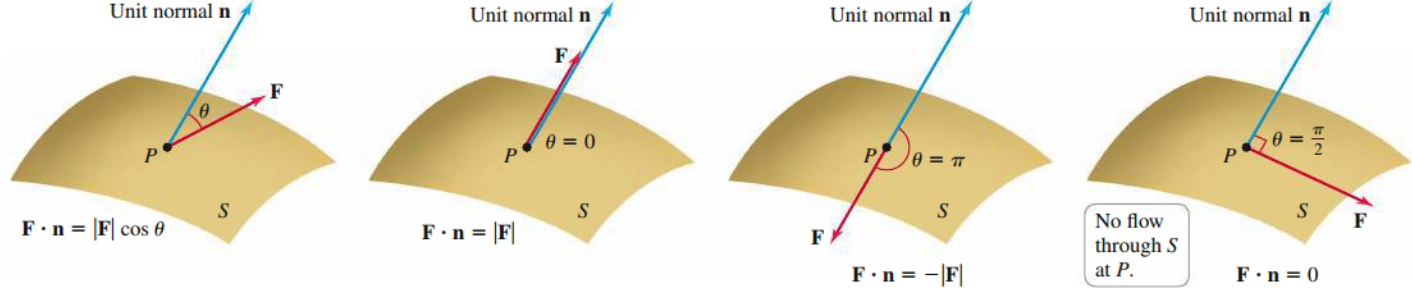
\includegraphics[width=0.95\linewidth]{images/briggs_17_06/fig17_57}
  \end{center}
  The unit normal vector we use is
    \[\vecn=\frac{\mathbf t_u\times\mathbf t_v}{\abs{\mathbf t_u\times\mathbf t_v}}\]
  giving us
    \begin{align*}
      \iint\limits_S \mathbf F\cdot\vecn\,dS&= \iint\limits_R \mathbf F\cdot\vecn \abs{\mathbf t_u\times\mathbf t_v}\,dA\\
      &= \iint\limits_R \mathbf F\cdot\frac{\mathbf t_u\times\mathbf t_v}{\abs{\mathbf t_u\times\mathbf t_v}} \abs{\mathbf t_u\times\mathbf t_v}\,dA\\
      &= \iint\limits_R \mathbf F\cdot\parens{\mathbf t_u\times\mathbf t_v}\,dA
    \end{align*}
  When the surface $S$ is explicitly given as $z=s(x,y)$, then 
    \[\mathbf F\cdot\parens{\mathbf t_u\times\mathbf t_v}=-fz_x-gz_y+h\]
  \pagebreak

  \begin{defn*}[Surface Integral of a Vector Field]
    Suppose $\mathbf F=\bracket{f,\,g,\,h}$ is a continuous vector field on a region of $\bbr^3$ containing a smooth oriented surface $S$. If $S$ is defined parametrically as $\vecr(u,v)=\bracket{x(u,v),\,y(u,v),\,z(u,v)}$, for $(u,v)$ in a region $R$, then
      \[\iint\limits_S \mathbf F\cdot\vecn\,dS=\iint\limits_R \mathbf F\cdot\parens{\mathbf t_u\times\mathbf t_v}\,dA,\]
    where $\ds\mathbf t_u=\frac{\partial \vecr}{\partial u}=\bracket{\frac{\partial x}{\partial u},\,\frac{\partial y}{\partial u},\,\frac{\partial z}{\partial u}}$ and $\ds\mathbf t_v=\frac{\partial \vecr}{\partial u}=\bracket{\frac{\partial x}{\partial v},\,\frac{\partial y}{\partial v},\,\frac{\partial z}{\partial v}}$ are continuous on $R$, the normal vector $\mathbf t_u\times\mathbf t_v$ is nonzero on $R$, and the direction of the normal vector is consistent with the orientation of $S$. If $S$ is defined in the form $z=s(x,y)$, for $(x,y)$ in a region $R$, then
      \[\iint\limits_S \mathbf F\cdot\vecn\,dS=\iint\limits_R \parens{-fz_x-gz_y+h}\,dA.\]
  \end{defn*}
  \pagebreak

  \begin{ex*}
    Consider the vertical field $\mathbf F=\bracket{0,0,-1}$. Find the flux in the downward direction across the surface $S$, which is the plane $z=4-2y-y$ in the first octant.
  \end{ex*}
  \begin{flushright}
    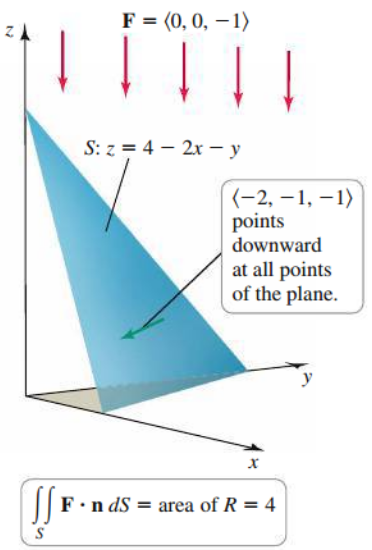
\includegraphics[width=0.25\linewidth]{images/briggs_17_06/fig17_58}
  \end{flushright}
  \vspace*{\stretch{1}}
  \pagebreak

  \begin{ex*}
    Consider the radial vector field $\mathbf F=\bracket{f,\,g,\,h}=\bracket{x,\,y,\,z}$. 
  \end{ex*}
  \begin{tasks}[after-item-skip=\stretch{1}, label=](1)
    \task 
    \task 
  \end{tasks}
  \vspace*{\stretch{1}}
  \pagebreak

\end{document}